

\setcounter{section}{4}
\section{Electrical Design}
\bigskip

\subsection{Power Management}

\pagebreak
\subsection{RF Harvester}
\medskip
Radio Frequency is an abundant source for energy harvesting especially in a radio wave rich environment. When Radio Waves reach an antenna it causes a changing potential difference across the antenna. The potential difference causes charge carriers to move along the length of the antenna in an attempt to equalize the field, and the RF-to-DC integrated circuit (Figure \ref{rf_bd}) is able to capture energy from the movement of those charge carriers. The energy is stored temporarily in a capacitor and then used to create a desired potential difference at the load \cite{R5-2-1}.

\medskip
\begin{figure}[H]
\centering
    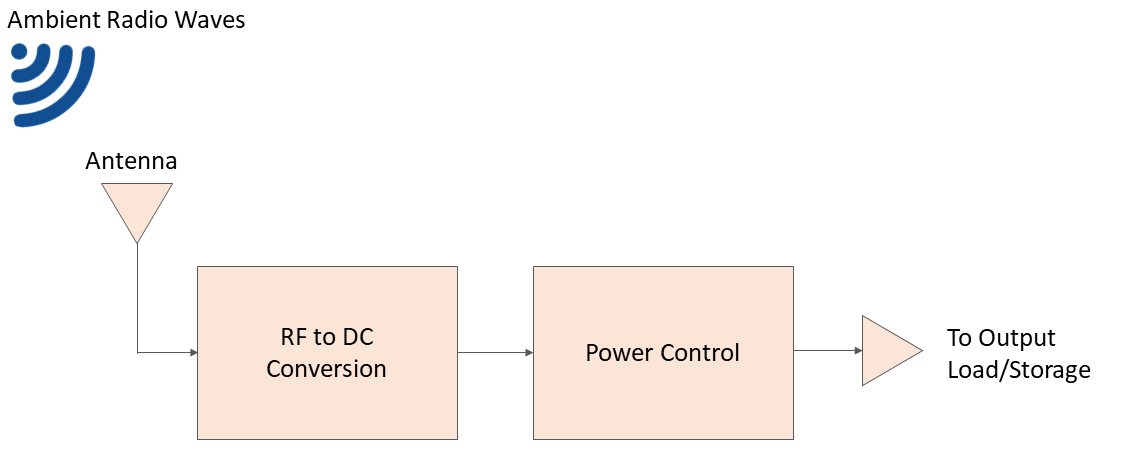
\includegraphics[scale=0.55]{./images/RF_H.png}
    \caption{RF Harvester Block Diagram}
    \label{rf_bd}
\end{figure}

There will be a demonstrable RF harvester circuit similar to Figure \ref{rf_c} that would convert ambient radio signal to DC voltage to charge the ID tag under deep sleep mode. During initial testing, the harvesting was able to collect up to 100 mV, however the ESP32 deep sleep mode requires 10 uA. Load calculation and capacitance optimization will need to be performed to further improve the reliability of the harvester. Once RF harvester test circuit produces adequate results in the prototype phase, the circuit will be implemented onto the ID Tag devices as PCB components. The RF harvester circuit designed for charging the ID tags will be collecting ambient RF power created from Wi-Fi and cellular communications to maintain charge for ESP32 during deep sleep mode.

\medskip
\begin{figure}[H]
\centering
    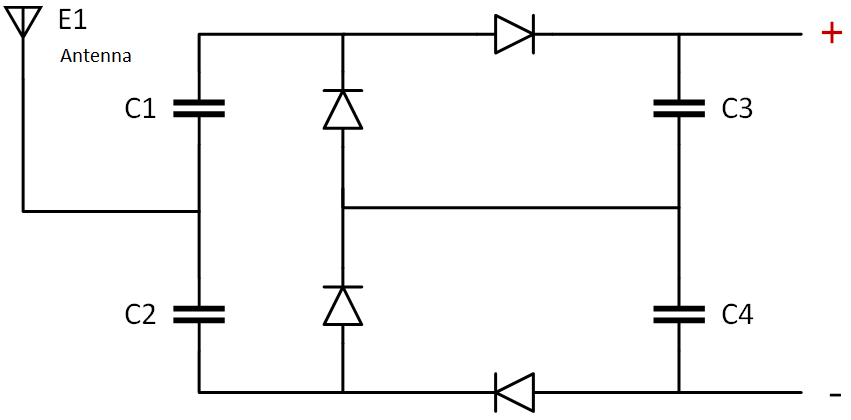
\includegraphics[scale=0.5]{./images/rf_circuit.png}
    \caption{RF Harvester Circuit Diagram}
    \label{rf_c}
\end{figure}



\pagebreak
\subsection{Electrical Design Requirements}
